
\noindent Continuing on the introduction to Hamiltonian lattice gauge theory as a means of quantization of gauge fields, we will build a microscopic formulation of gauge theory based on the real-space lattice. In contrast to the usual way of working on the Euclidean, Wick-rotated lattices, we will begin our theory with a Hamiltonian of classical degrees of freedom: namely, the parallel transporter $U$, a $2 \times 2$ matrix with determinant one, such that $U \in SU(2)$. Since we are working in 4D spacetime, we will have a 4D discretized lattice with lattice spacing $a \propto \frac{1}{K_c}$. In other words, 4D spacetime is discretized up to the cutoff $K_c$. \\ 

\noindent Like introduced before, each link, or edge, of the lattice $e \in E$, where $E$ is the set of all links of the lattice, has an associated parallel transporter, corresponding to the shortest, rectilinear path in between each vertex, $U_e \in SU(2) \simeq S^3$. Note that the parallel transporter is not a local object, as it is path dependent, implicitly depending on more than one coordinate. \\

\noindent The classical configuration space for this lattice gauge theory is a Cartesian product of $SU(2)$ per link in the lattice

\begin{equation}
\mathcal{C} = SU(2) \times SU(2) \times \dots \times SU(2).
\end{equation}

\noindent To quantize this classical lattice gauge theory, we'll begin by taking the simplest guess possible and introduce a wavefunction $\psi: \,\, \mathcal{C} \rightarrow \mathcal{C}$, where the Hilbert space has a ket basis $\ket{\psi} \in \mathcal{H} \simeq \otimes_{e \in E} h_e$, where $h_e$ is the space over each link. \\

\noindent Since $SU(2)$ is diffeomorphic to $S^3$, we are hinted towards defining wavefunctions as square-integrable functions on a sphere, and each point on the sphere will be associated to a complex number. Therefore, we define $h_e \equiv L^2(SU(2))$, where $L^2(SU(2))$ is an infinite-dimensional separable Hilbert space, since there are arbitrarily many orthogonal wavefunctions defined on the sphere. \\

\noindent Recall the two operators defined in $SU(2)$, for unitary matrix with unit determinant $U \in SU(2)$, that defined a right- and left-acting transformation

\begin{align}
&L_U : \,\, L^2 (SU(2)) \rightarrow L^2 (SU(2)) \\
&R_U : \,\, L^2 (SU(2)) \rightarrow L^2 (SU(2))
\end{align}

\noindent Where $L_U$ and $R_U$ commute, such that $[L_U, R_U]=0$, and form the representation defined by the relations 

\begin{equation}
L_U^\dagger L_U = R_U^\dagger R_U = \mathbb{I} \text{ and } L_{UV} = L_U L_V.
\end{equation}

\noindent To understand how the infinite-dimensional Hilbert space $L^2(SU(2))$ breaks up into a direct sum of irreducible representations of $SU(2)$, we invoke the third part of the \textit{Peter-Weyl therorem}, which states that the Hilbert space over $SU(2)$ consisting of square-integrable functions may be regarded as a representation of a direct product of left- and right-acting operators, and the Hilbert space decomposes into an orthogonal direct sum of all the irreducible unitary representations, with multiplicity of each irreducible representation equal to its degree, the dimension of the underlying space of that representation (See Wikipedia page on Peter-Weyl theorem for overview). We write this all as \\

\begin{equation}
h_e \equiv L^2(SU(2)) \simeq \bigoplus_{l \in \frac{1}{2}\mathbb{Z}^+} \,\, V_l \otimes V_l^* \simeq \bigoplus_{l \in \frac{1}{2}\mathbb{Z}^+} \,\, \mathbb{C}^{2l+1} \otimes \mathbb{C}^{2l+1}
\end{equation}

\noindent Where $V_l \simeq \mathbb{C}^{2l+1}$ is the $(2l+1)$-dimensional vector space furnishing the irreducible representation of $SU(2)$ of spin, or angular momentum $l$ and $\frac{1}{2}\mathbb{Z}^+ = \{0,\frac{1}{2},1,\frac{3}{2},2,\dots\}$. \\

\noindent Now to find a representation of $SU(2)$ on this vector space $V_l$, we'll use a piece of Lie group representation theory not found in any textbook. Note that the action of $SU(2)$ generates a representation

\begin{equation}
\Pi_l (SU(2)) : \,\, V_l \rightarrow V_l.
\end{equation}

\noindent In the procedure to calculate the matrix $\Pi_l (SU(2))$, we will use two pieces of machinery

\begin{itemize}
\item The spin-$\frac{1}{2}$ fundamental representation of $SU(2)$
	\subitem $\Pi_{\frac{1}{2}} (U) = \left(\begin{array}{cc} a & b \\ c & d \end{array}\right)$
\item Tensor products of the spin-$\frac{1}{2}$ 2D vector spaces furnishing the fundamental representation of $SU(2)$, $V_{\frac{1}{2}} \simeq \mathbb{C}^2 \equiv \{ \ket{0}, \ket{1} \}$.
\end{itemize}

\noindent Begin the procedure to get the matrix representation for any spin-$l$, take the tensor product of $n$ of the spin-${\frac{1}{2}}$ fundamental vector spaces 

\begin{equation}
V_{\frac{1}{2}} \otimes V_{\frac{1}{2}} \otimes \dots \otimes V_{\frac{1}{2}}.
\end{equation}

\noindent Note that for quantum computer fans, this is the vector space of $n$ qubits

\begin{equation}
V_{\frac{1}{2}} \otimes V_{\frac{1}{2}} \otimes \dots \otimes V_{\frac{1}{2}} \simeq \mathbb{C}^2 \otimes \dots \otimes \mathbb{C}^2 = \mathcal{C}^{2^n}.
\end{equation}

\noindent The spin-$l$ representation $\Pi_l(U)$, generated from $SU(2)$ action on $V_l$, lives in thsi tensor product space of $n$ copies of $V_{\frac{1}{2}}$, as long as $n=2l$ or $l=\frac{n}{2}$. Therefore, we will build $V_l$ as a subspace of this tensor product space, most fo which will be thrown away once we find our subspace of interest, by building a set a $n+1$ orthonormal vectors

\begin{align}
\ket{w_{\frac{n}{2}}} &= \ket{1 1 \dots 1} \\
\ket{w_{\frac{n}{2}-1}} &= \frac{1}{\sqrt{n}} \left( \ket{1 1 \dots 1 0} + \ket{1 1 \dots 1 0 1} + \dots + \ket{0 1 \dots 1} \right) \\
\dots& \\
\ket{w_{\frac{n}{2}-k}} &= \frac{1}{\sqrt{n \choose k}} \left( \ket{ 1 \dots 1 0 \dots 0} + \text{(all permutations of $k$ zeros and $n-k$ ones)} \right) \\
\dots& \\
\ket{w_{-\frac{n}{2}}} &= \ket{ 0 0 \dots 0}.
\end{align}

\noindent Then the matrix elements of the representation $\Pi_l (U)$ are simply given by the expectation value on $n$ copies of $U$ in this orthonormal basis

\begin{equation}
[\Pi_l (U) ]_{jk} = \bra{w_j} U \otimes \dots \otimes U \ket{w_k}
\end{equation}

\noindent Where $j, \, k \in \{ -\frac{n}{2}, \dots, \frac{n}{2} \}$. \\

\noindent Note that this method is good and fast for low spin representations, but clearly gets unwieldy for working with the Hilbert space of $n=1000$ qubits, and the efficiency and value of the methods of addition of angular momentum and Clebsch-Gordan coefficients, with the raising and lower operators, the highest-weight vectors, etc. \\

\noindent Sticking to low spin representations for our purposes, we can start to extract matrix representations for $l=0$, $l=\frac{1}{2}$, and $l=1$. \\

\noindent For $l=0$, the matrix representation is just the identity

\begin{equation}
\Pi_0 (U) = \mathbb{I}.
\end{equation}

\noindent For $l=\frac{1}{2}$, we have the fundamental matrix representation 

\begin{equation}
[\Pi_{\frac{1}{2}} (U) ]_{jk} = [U]_{jk}.
\end{equation}

\noindent In the $l=1$ subspace, there are three orthonormal basis vectors

\begin{equation}
\{ \ket{w_1} = \ket{1 1}, \,\, \ket{w_0} = \frac{1}{\sqrt{2}} (\ket{1 0} + \ket{0 1}), \,\, \ket{w_{-1}} = \ket{0 0} \}.
\end{equation}

\noindent The matrix elements are then gotten by the expectation value above, pulling values from the fundamental representation

\begin{align}
[\Pi_1 (U) ]_{11} &= \bra{1 1} U \otimes U \ket{1 1} = \bra{1} U \ket{1} \bra{1} U \ket{1} = a^2 \\
[\Pi_1 (U) ]_{00} &= \frac{1}{2} \left( \bra{1 0} U \otimes U \ket{1 0} + \bra{1 0} U \otimes U \ket{0 1} + \bra{0 1} U \otimes U \ket{1 0} + \bra{0 1} U \otimes U \ket{0 1} \right) \\
 &= ad + bc.
\end{align}

\noindent Recall that the Peter-Weyl theorem tells us that the Hilbert space of square-integrable functions on $SU(2)$ is isomorphic to the infinite-dimensional, until we truncate, direct sum space of $(2l+1)$-dimensional vector spaces furnishing the representation of $SU(2)$

\begin{equation}
L^2 (SU(2)) \simeq \bigoplus_{l \in \frac{1}{2}\mathbb{Z}^+} \,\, \mathbb{C}^{2l+1} \otimes \mathbb{C}^{2l+1}.
\end{equation}

\noindent And $SU(2)$ acts on $L^2 (SU(2))$ via the operator $L_U: \, L^2 (SU(2)) \rightarrow L^2 (SU(2))$ with action

\begin{equation}
L_U \simeq \bigoplus_{l \in \frac{1}{2}\mathbb{Z}^+} \,\, \Pi_l (U) \otimes \mathbb{I}.
\end{equation}

\noindent The elements of the matrix representation $[\Pi_l (U)]_{jk} \equiv t^l_{jk} (U)$ are square-integrable functions from $SU(2)$ to the complex numbers $\mathbb{C}$, since $SU(2)$ is compact, and form an orthogonal (not orthonormal) basis for $L^2 (SU(2))$, where $-l \le j,k \le l$. So, we can expand the wavefunction ket in the orthogonal basis of the matrix elements

\begin{equation}
\ket{\psi} = \sum_l \sum_{j,k} \psi^l_{jk} \ket{j}_l \ket{k}_l = \sum_l \sum_{j,k} \psi^l_{jk} \sqrt{2l+1} \ket{t^l_{jk}}.
\end{equation}

\noindent The inner product of the Hilbert space $L^2 (SU(2))$ is defined with the Haar measure $\int dU$ by

\begin{equation}
(\psi, \phi) \equiv \int dU \, \psi^* (U) \phi(U)
\end{equation}

\noindent Where we use the inner product of the orthogonal basis vectors, where integrals over $SU(2)$ with the Haar measure behave like $\int dU \, U \otimes U^\dagger \propto \mathbb{I} \otimes \mathbb{I} + (\text{swap operations})$, and (\textbf{Exercise})

\begin{equation}
(t^l_{jk}, t^{l'}_{j'k'}) = \delta^{ll'} \delta_{jj'} \delta_{kk'} \frac{1}{2l+1}.
\end{equation}

\noindent Therefore, the basis for the total Hilbert space consists of wavefunctions $\ket{\Psi} \in \mathcal{H}$ and

\begin{equation}
\ket{\Psi} = \sum_{l_1 l_2 \dots} \sum_{j_1 j_2 \dots} \sum_{k_1 k_2 \dots} \, \Psi^{l_1 l_2 \dots}_{j_1 j_2 \dots k_1 k_2 \dots} \ket{j_1}_{l_1} \ket{k_1}_{l_1} \ket{j_2}_{l_2} \ket{k_2}_{l_2} \dots .
\end{equation}

\noindent To give dynamics to the Hilbert space, we define some observables. Consider an element of $SU(2)$, $U=e^{c_j \tau^j}$, where $c_j \tau^j$ are elements of the Lie algebra of $SU(2)$, $c_j \in \mathbb{R}^3$, and $\tau^j$ are the Pauli spin matrices multiplied by i and divided by 2 for normalization conditions. The spin matrices obey the commuation relations $[\tau^j,  \tau^k] = -2 \epsilon^{jk}_{\,\,\,\,l} \tau^l$. We can recover the spin matrix from the group element via differentation

\begin{equation}
\frac{d U}{d c_j} \Big{|}_{c_j = 0} = \tau^j.
\end{equation}

\noindent The first observable we define is the anti-Hermitian \textit{left angular momentum operator}

\begin{equation}
\hat{l}_L^j \equiv \frac{d}{ds} L_{U=e^{s\tau^j}} \Big{|}_{s=0}.
\end{equation}

\noindent Note that this is a factor of $i$ away from being Hermitian, and is analogous to the Hermitian linear momentum operator $i\hat{p}$. Also, notice that we begin with a unitary operator $L_U$, apply an anti-Hermitian operator $\frac{d}{ds}$, and kill off the unitarity by setting $s=0$ after the derivative. \\

\noindent The second observable we define, similar to the first, is the \textit{right angular momentum operator}

\begin{equation}
\hat{l}_R^j \equiv \frac{d}{ds} R_{U=e^{s\tau^j}} \Big{|}_{s=0}.
\end{equation}

\noindent Next, define the position observable $\hat{U}_{jk}$, which is also a map $L^2 (SU(2)) rightarrow L^2 (SU(2))$ and yields the fundamental representation matrix elements when it acts on the position eigenkets $\ket{U}$ of $SU(2)$.

\begin{equation}
\hat{U}_{jk} \ket{U} = [\Pi_{\frac{1}{2}} (U) ]_{jk} \ket{U}.
\end{equation}

\noindent Acting the position operator on the Hilbert space wavefunctions $\ket{\psi} = \int dU \, \psi(U) \ket{U}$, we get the Haar integral over position eigenkets

\begin{equation}
\hat{U}_{jk} \ket{\psi} = \int dU \, \psi(U) [\Pi_{\frac{1}{2}} (U)]_{jk} \ket{U} = \int dU \, \psi(U) t^{l=\frac{1}{2}}_{jk} (U) \ket{U}.
\end{equation}

\noindent To build the Hamiltonian, kinetic energy plus potential energy, we use the plaquette operator to define parallel transport on the 4D lattice

\begin{align*}
\hat{U}_\Box : \,\, &L^2 (SU(2)) \otimes L^2 (SU(2)) \otimes L^2 (SU(2)) \otimes L^2 (SU(2)) \\
&\rightarrow L^2 (SU(2)) \otimes L^2 (SU(2)) \otimes L^2 (SU(2)) \otimes L^2 (SU(2))
\end{align*}

\noindent We choose the convention to set arrows on each link running ``left-to-right'' and ``down-to-up'' in the plane of the ``paper'', and then walk around the plaquette counterclockwise (CCW), taking the Hermitian conjugate of the parallel transporter if we are traveling against the arrow. The parallel transporter for each link is considered the observable for that link when traveling around the plaquette. Each link are labeled by $e_i$, $i=1,2,3,4$. \\

\begin{figure}[H]
	\centering
	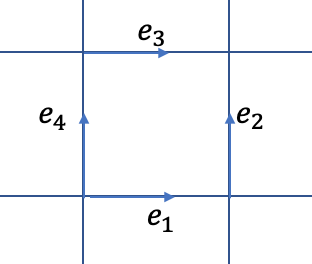
\includegraphics[width=1.5in]{images/ks_plaquette.png}
	\caption*{}
\end{figure}

\noindent Build an operator that acts on the 4D space of links, as a sum over the links of the direct products of parallel transporters

\begin{equation}
\hat{M}_{\Box; j_1, k_4} = \sum_{k_1, k_2, k_3} \hat{U}_{j_1 k_1} \otimes \hat{U}_{k_1 k_2} \otimes \hat{U}_{k_2 k_3}^\dagger \otimes \hat{U}_{k_3 k_4}^\dagger.
\end{equation}

\noindent This is then turned into an observable by summing over the last, initially-fixed index $k_4$

\begin{equation}
tr(\hat{U}_\Box) \equiv \sum_{k_4} \hat{M}_{\Box; k_4, k_4}.
\end{equation}

\noindent Note that $tr(\hat{U}_\Box)$ is a trace operator that acts on $L^2 (SU(2)) \otimes L^2 (SU(2)) \otimes L^2 (SU(2)) \otimes L^2 (SU(2))$, and \textbf{not} a number! \\

\noindent Put the defined observables together into the \textit{Kogut-Susskind Hamiltonian}

\begin{equation}
\hat{H}_{KS} = -\frac{g_H^2}{2a} \sum_{e \in E} \, \hat{l}_L^j (e) \hat{l}_L^j (e) + \frac{1}{2 g_H^2 a} \sum_{\text{plaquettes } \Box} \, \left(tr(\hat{U}_\Box) + \text{Hermitian conjugate} \right)
\end{equation}

\noindent Where $g_H$ is the coupling constant. \\

\noindent This model has a huge group of gauge symmetries. \\

\noindent Consider a vertex in the lattice and build the operator

\begin{figure}[H]
	\centering
	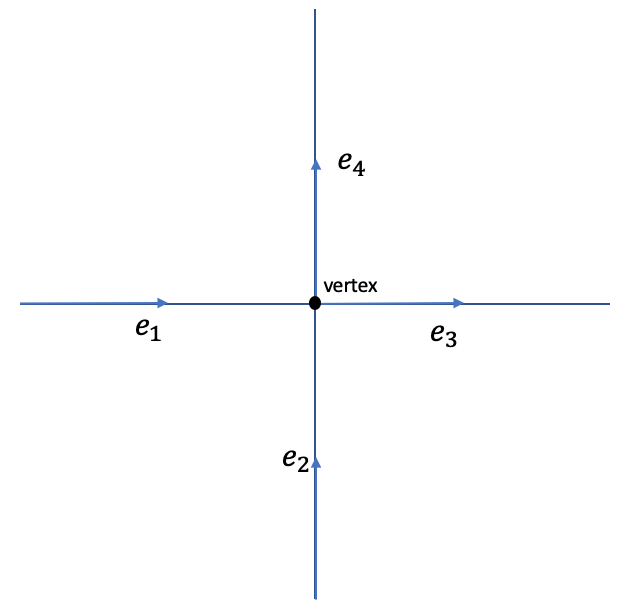
\includegraphics[width=1.5in]{images/ks_vertex.png}
	\caption*{}
\end{figure}

\begin{equation}
M_x \equiv R_x (e_1) \otimes R_x (e_2) \otimes L_x (e_3) \otimes L_x (e_4)
\end{equation}

\noindent Where $x \in SU(2)$. These operators obey the following commutation relations 

\begin{equation}
[M_x (v), M_y (w)] = 0 \text{ and } [M_x (v), \hat{H}_KS] = 0 \text{, for all } x, y, v, w.
\end{equation}

\noindent In summary, Wilson's formulation received much more attention at the time for its ease of discretizstion, translation to computer programs, and use of Monte Carlo sampling, which classical computers are good at. Kogut and Susskind argued that the plaquette operator becomes the curvature term, as expected, in the small lattice spacing $a$ limit in their theory, as well as that hte kinetic energy term becomes the kinetic energy in the timelike direction of the curvature term. The Kogut-Susskind formulation may be very promising for quantum simulations done by quantum computers, which are not very good at sampling techniques, but excel in simulating the dynamics of local lattice models.